
\documentclass{IIBproject}
\usepackage[utf8]{inputenc}

\usepackage{setspace}
\onehalfspacing

\usepackage{graphicx,float,epstopdf,subcaption}
\graphicspath{{method/}{method/gen}}

\makeatletter
\def\input@path{{method/}{method/gen}}
\makeatother

\usepackage{tikz,fp}
\usetikzlibrary{positioning,calc}

\definecolor{colorA}{rgb}{0.1686, 0.5137, 0.7294}
\definecolor{colorB}{rgb}{0.9922, 0.6824, 0.3804}
\definecolor{colorC}{rgb}{0.4706, 0.6745, 0.4392}
\definecolor{colorD}{rgb}{0.8431, 0.0980, 0.1137}

\usepackage{amsmath,amsfonts,bm,physics}
\newcommand{\vect}[1]{\bm{#1}}
\newcommand{\mat}[1]{\mathbf{#1}}
\newcommand{\dra}{\dashrightarrow}
\newcommand{\dla}{\dashleftarrow}
\newcommand{\acc}{{\mkern 0.5mu\cdot\mkern 0.5mu}}
\renewcommand{\O}[1]{\mathcal{O}(#1)}


\usepackage[section]{algorithm}
\usepackage{algpseudocode}
\algnewcommand\algorithmicsend{\textbf{send}}
\algnewcommand\Send{\State\algorithmicsend\ }
\algnewcommand\algorithmicrecv{\textbf{recv}}
\algnewcommand\Recv{\State\algorithmicrecv\ }
\algnewcommand\algorithmicgather{\textbf{gather}}
\algnewcommand\Gather{\State\algorithmicgather\ }
\algnewcommand\algorithmicscatter{\textbf{scatter}}
\algnewcommand\Scatter{\State\algorithmicscatter\ }
\algnewcommand\algorithmicforeach{\textbf{for\ each}}
\algblockdefx[ForEach]{ForEach}{EndFor}
[1][]{\algorithmicforeach\ #1}
{\textbf{end\ for}}

% \usepackage{minted,sourcecodepro}

\usepackage[backend=biber,bibstyle=alphabetic,citestyle=alphabetic]{biblatex}
\bibliography{refs}


\begin{document}

\date{14th November 2016}
\author{Matt Diesel (md639)}
\supervisor{Dr. Jie Li}
\title{Parallel Adaptation of Orthotree Meshes}

% \pagestyle{empty}
% \maketitle

% \thispagestyle{empty}
% \begin{abstract}
% Abstract
% \end{abstract}

% \tableofcontents
% \newpage
% \pagestyle{plain}


% \section{Introduction}

Hopefully already defined by this point:

\begin{itemize}
	\item $\mathbb{W} \in [0;W)$ the set of processes in the world. A processes rank is its index in the world.
	\item $p$ the rank of the current process
	\item A cell reference $\mathcal{C}$ that has a number of methods:
	\begin{itemize}
		\item $\mathcal{C}\acc\textproc{rank}$ - the rank owning the cell, uses the variable $\rho$ to denote.
		\item $\mathcal{C}\acc\textproc{data}$ - the data associated with the cell, uses the variable $\phi$ to denote.
		\item $\mathcal{C}\acc\textproc{ident}$ - the cells identifier, uses the variable $\lambda$ to denote. 
		\item A set of neighbours $\mathcal{C}\acc\vect{\mathcal{N}} = \{\mathcal{N}_0 , \mathcal{N}_1, \dots , \mathcal{N}_n\}$
		\item A space filling curve
	\end{itemize}
\end{itemize}


\section{Method}

\subsection{Orthotree Fundamentals}

An orthotree is an N dimensional tree structure, where each cell is orthotopic \cite{coxeter73} and its children are evenly sized similar orthotopes. For this project, the 2d case (known as a Quadtree) was implemented and examined in detail. Much of the code does not depend on the dimension however, and the algorithms extend into N dimensions easily.

We refine the tree depending on the conditions of the problem being solved. Figure \ref{fig:layeredtree} shows a simple case where we refine to a simple line geometry.

\begin{figure}[H]
	\caption{4 levels of a Quadtree refined to a line shown in blue. If a cell has children, they are shown in orange.}
	\label{fig:layeredtree}
	

\begin{tikzpicture}
    \newcommand\topLayer{3}

    \begin{scope}[
        yshift=0,every node/.append style={
        yslant=0.5,xslant=-1},yslant=0.5,xslant=-1]
        \draw[black,very thick] (0,0) rectangle (4,4);

        % \begin{scope}[every node/.append style={}]
        %     \foreach \i in {\topLayer,...,0} {
        %         \input{layer\i-t0}
        %     }
        % \end{scope}
        \input{mesh-t0}

        % y = 0.3 + 6.189086*x - 6.682936*x^2 + 2.481516*x^3 - 0.2852701*x^4
        \draw[domain=0:3.8,smooth,variable=\x,colorA, ultra thick] plot ({\x},
            {0.3 + 6.189086*\x - 6.682936*\x*\x + 2.481516*\x*\x*\x - 0.2852701*\x*\x*\x*\x});

    \end{scope} %end of drawing grids
    \node[anchor=west,text width=7cm] at (5cm,2cm) {The resultant mesh is comprised of all the cells without children - the "leaves" of the tree.};
        
    \foreach \i in {\topLayer,...,0} {
        \begin{scope}[
            yshift=5cm+2cm*(\topLayer-\i),every node/.append style={
                yslant=0.5,xslant=-1},yslant=0.5,xslant=-1
              ]
            \fill[white,fill opacity=0.9] (0,0) rectangle (4,4);
            % y = 0.3 + 6.189086*x - 6.682936*x^2 + 2.481516*x^3 - 0.2852701*x^4
            \draw[domain=0:3.8,smooth,variable=\x,colorA, thin] plot ({\x},
                {0.3 + 6.189086*\x - 6.682936*\x*\x + 2.481516*\x*\x*\x - 0.2852701*\x*\x*\x*\x});

            \ifnum \i=\topLayer
            \else
                \FPeval{\result}{round(\i+1, 0)}%
                \begin{scope}[every node/.append style={colorB}]
                    \input{layer\result-t0}
                \end{scope}
            \fi

            \input{layer\i-t0}
            \draw[black,very thick] (0,0) rectangle (4,4);

        \end{scope}

        \node[yshift=7cm+2cm*(\topLayer-\i), anchor=west,text width=6cm] at (5cm,0) {Level \i};
    }
\end{tikzpicture}

\end{figure}

Although cells are stored at all levels in order to make tree traversal possible and ease refinement or coarsening of cells, processing of the problem is only done on the finest possible level. The set of cells without children make up the leaves of the tree $\mathbb{L}$ and it is this set that is of interest. The number of cells in the tree is written as $\abs{\mathbb{L}}$.

However, the refinement in Figure \ref{fig:layeredtree} is based on the assumption that the cells of interest are only those directly on the line. In reality, we spread the refinement levels such that for all cells, there are no cells within a parameter $P$ cell widths in the axis directions that are more than 1 level apart. This is called refinement propagation, examples of which are presented in Figure \ref{fig:refprop}.

The case $P=1$ is known as Two to One Balancing, as a cell has no neighbours more than twice its size. Since the term balancing is used to refer to parallel load balancing in this report, this term will be avoided. 

\expandafter\newcommand\csname countL(0) \endcsname{280}
\expandafter\newcommand\csname countL(1) \endcsname{452}
\expandafter\newcommand\csname countL(2) \endcsname{604}
\newcommand{\getCount}[1]{\csname countL(#1) \endcsname}

\begin{figure}[H]
\centering
\foreach \i in {0,1,2} {
	\begin{subfigure}{.3\textwidth}
	  \centering
		\begin{tikzpicture}
	        \draw[domain=0:3.8,smooth,variable=\x,colorA, thick] plot ({\x},
	            {0.3 + 6.189086*\x - 6.682936*\x*\x + 2.481516*\x*\x*\x - 0.2852701*\x*\x*\x*\x});
			\input{method/gen/mesh-t\i}
		\end{tikzpicture}
	  \caption{\\ $P=\i$ \\ $\ \ \abs{\mathbb{L}}=\getCount{\i}$}
	  \label{fig:refprop-t\i}
	\end{subfigure}%
}
\caption{Meshes for various refinement propagation levels $P$ to the example line geometry. In all cases the maximum refinement level is $5$, giving an equivalent uniform mesh cell count of $1024$ cells.}
\label{fig:refprop}
\end{figure}

\subsection{Fully Threaded Trees}

The use of orthotree structures in Adaptive Mesh Routines was proposed by Khokhlov in \cite{Khokhlov98}. To tailor them towards solving the differential equation in fluid problems, his implementation included linking cells to all their neighbours to allow $\mathcal{O}(1)$ lookup compared to a possible $\mathcal{O}(\log n)$ lookup using tree traversal. Khoklov termed the tree with the neighbour pointers a Fully Threaded Tree (FTT) structure. 

In \cite{Khokhlov98}, an optimisation is presented to reduce the memory overhead introduced by storing neighbour pointers by noting that for (in the quadtree case) the children of a cell, half the neighbours are also children of that cell. By storing groups of children together in an ortho (referred to as a quad in 2d and octo in 3d) the memory requirement for storing neighbour links is almost halved.



\subsection{Threaded FTT}


\subsection{Global Identifiers}

To enable inter-process communication, a cell identifier format is required that is guaranteed to be unique within the tree. Furthermore, the identifier must be constant for the same cell existing on multiple processes. 

The identifier of a cell is accessed as $\mathcal{C}\acc\textproc{ident}$. Two functions are required for finding (\ref{fun:find}) and inserting (\ref{fun:insert}) the cell with a given identifier $\lambda$ into the tree.

\begin{align}
	\label{fun:find}
	\textproc{Find}(\lambda) \mapsto \mathcal{C} \\
	\label{fun:insert}
	\textproc{Insert}(\lambda) \mapsto \mathcal{C}
\end{align}

The implementation chosen for this project encodes both the level and location of the cell as an unsigned integer, hence uniquely identifying it within the entire tree, and allowing logarithmic lookup and insertion times. Retrieving the level, child and parent identifiers, or the child index of the cell is done with bitwise arithmetic. 

The most significant byte of the integer encodes the level. The remainder of the bits encodes the child orthant for each successive step down the tree with the highest level being in the least significant bits. The number of bits needed to encode an orthant is equal to the number of dimensions of the problem. Using a 64 bit integer this allows for a maximum tree depth of 28 levels in a quadtree, or 18 octree levels. 


\subsection{Poisson Neighbourhoods}

To solve on the adaptive mesh, interpolation is required in cases where the level of adjacent cells do not match. It is possible to move the expensive interpolation operation outside of the tight solver loop by instead storing a list of cells required along with the co\"efficient they would have been scaled by using direct interpolation. This list of cells is known as the poisson neighbourhood for a cell $\mathcal{C}$ and is represented by the vector $\mathcal{C}\acc\vect{\mathcal{P}}$. The respective neighbour co\"efficients are represented by the vector $\mathcal{C}\acc\vect{\beta}$ and the central co\"efficient is a scalar $\mathcal{C}\acc\alpha$. 

The poisson neighbourhood is important for cells close to the border between processes, as it represents the necessary set of cells to perform the calculations. 

Calculating the co\"efficients for the different cases is explored in detail by \cite{Yung2010} including for higher order solvers. The methods used here are independent of the order of the solver, and the determining the neighbourhood is abstracted to Function \ref{fun:CalcPoisCoefs}. 

\begin{equation}
	\label{fun:CalcPoisCoefs}
	\textproc{CalcPoisCoefs}(\mathcal{C}) \mapsto \{ \vect{\mathcal{P}}, \vect{b}, \alpha \}
\end{equation}

\subsection{Ghosts and Borders}
\label{sec:ghostsandborders}

For each process near its boundaries there are cells who require the data from poisson neighbours outside the tree of the process. These are known as ghost cells, and in order to solve in parallel their values must be retrieved at each iteration. For a process $x$ the set of ghost cells whose rank is another process $y$ is written as $\mathbb{G}_y$. 

Each process also stores the set of cells it owns, who are ghost cells of foreign processes. These are called the border cells, and for a process $x$ the set of border cells to another process $y$ is written as $\mathbb{B}_y$.

A good space filling curve, such as the Hilbert Curve, leads to process' cells being closely grouped and close to square, for example the 3 processes in Figure \ref{fig:borderline} are grouped reasonably well with few peninsulas. 

\begin{figure}[H]
	\caption{Border cells for 3 processes}
	\label{fig:borderline}
	\input{method/gen/borderline.tex}
\end{figure}

For rank zero, there are ghost cells on both of the other processes as shown in Figure \ref{fig:borders-r0}. 

\begin{figure}[H]
	\caption{Ghost cells for rank 0}
	\label{fig:borders-r0}
	\input{method/gen/ghosts-r0.tex}
\end{figure}

A highly desirable property of the border and ghost sets that greatly simplifies the retrieval of ghost cell data is that for any two processes $x$ and $y$, $\mathbb{G}_y$ on $x$ is exactly the same as $\mathbb{B}_x$ on $y$. In order to guarantee that property the sets are kept sorted according the the global identifier. 

Individual processes do not have enough information to generate their own ghost sets. As a result, the ghost sets for all processes is transferred with the initial cell distribution as outlined in Section \ref{sec:distribution}. However, knowledge of a processes own cell and ghost sets is sufficient to generate the border set using the method in Algorithm \ref{alg:borders-gen}.

\begin{algorithm}[H]
\caption{Building the border set on process $p$}
\label{alg:borders-gen}

\begin{algorithmic}
\Require A complete ghost set $\mathbb{G}$ for the process $p$.
\Statex
\State $\mathbb{B} \gets \emptyset$
\ForEach {ghost cell $\mathcal{G} \in \mathbb{G}$}
	\ForEach {poisson neighbour $\mathcal{P} \in \mathcal{G}\acc\vect{\mathcal{P}}$}
		\If {$\mathcal{P}\acc\textproc{rank} = p$}
			\State $\mathbb{B}_{\mathcal{G}\acc\textproc{rank}} \gets \mathcal{P}$
		\EndIf
	\EndFor
\EndFor
\end{algorithmic}
\end{algorithm}


\subsection{Distribution}
\label{sec:distribution}

Initial distribution is performed as a single process. The tree is refined to its initial mesh, typically according the the known geometry of the problem. The number of cells to be allocated to each process is calculated by dividing the cell count for the initial tree by the number of processes. The procedure in Algorithm \ref{alg:distrib-assign} then iterates over the space filling curve, setting cells to the current value of a rank counter and incrementing the counter when the processes cell count is reached.

\begin{algorithm}[H]
\caption{Building the border set on process $p$}
\label{alg:distrib-assign}

\begin{algorithmic}
\Require An initialised complete tree $\mathbb{L}$
\Statex
\State $\bar{c} \gets \frac{\abs{\mathbb{L}}}{\abs{\mathbb{W}}}$ \Comment {Cells per rank}
\State $\rho \gets 0$ \Comment {Rank counter}
\State $c \gets \bar c$ \Comment {Cell count remaining for the current rank}
\ForEach {cell $\mathcal{C} \in \mathbb{L}$ in SFC order}
	\State $\mathcal{C}\acc\textproc{rank} \gets \rho$
	\State $c \gets c-1$
	\If {c = 0} \Comment {Step onto the next rank}
		\State $\rho \gets \rho+1$
		\State $c \gets \bar c$
	\EndIf
\EndFor
\end{algorithmic}
\end{algorithm}

Since it is not possible for a process to determine its own set of ghost cells without more knowledge of the tree, the starting process then generates all the ghost sets for every rank by using the poisson neighbourhood. 

\begin{algorithm}[H]
\caption{Generating the ghost sets for all processes}
\label{alg:distrib-ghosts}

\begin{algorithmic}
\Require An initialised complete tree $\mathbb{L}$, with cell ranks assigned for every leaf.
\Ensure A complete ghost set $\mathbb{G}_{\rho\gets b}$, for every pair of processes $\rho$ and $b$
\Statex
\State $\mathbb{G} \gets \emptyset$
\ForEach {leaf $\mathcal{C} \in \mathbb{L}$}
	\ForEach {poisson neighbour $\mathcal{P} \in \mathcal{C}\acc\vect{\mathcal{P}}$}
		\If {$\mathcal{P}\acc\textproc{rank} \neq \mathcal{C}\acc\textproc{rank}$}
			\State $G_{\mathcal{C}\acc\textproc{rank}\gets\mathcal{P}\acc\textproc{rank}} \gets \mathcal{P}$
		\EndIf
	\EndFor
\EndFor

\end{algorithmic}
\end{algorithm}

The tree is then serialised into a list for every process $\vect{N}_p=\{\lambda,\rho\}^n$ containing pairs of cell identifiers $\lambda$ and ranks $\rho$ referring to either an active cell or a ghost cell of the target process. These are sent to the processes, which unpack them according to the logic in Algorithm \ref{alg:distrib-unpack}.

\begin{algorithm}[H]
\caption{Building the subset of the tree on process $p$}
\label{alg:distrib-unpack}

\begin{algorithmic}
\Require A list $\vect{\hat N}=\{\lambda,\rho\}^n$ containing the cells required by this process.
\Statex
\State $\mathbb{G} \gets \emptyset$ \Comment{Ghost set is initially empty}
\ForEach {packed cell $\{\lambda,\rho\} \in \vect{\hat N}$}
	\State $\mathcal{C} \gets \textproc{Insert}(\lambda)$ \Comment{$\mathcal{C}$ is a temporary cell reference}
	\State $\mathcal{C}\acc\textproc{rank} \gets \rho$
	\If {$\rho \neq p$} \Comment {$\mathcal{C}$ must be a ghost if its rank is not the current process}
		\State $\mathbb{G}_\rho \gets \mathcal{C}$ 
	\EndIf
\EndFor
\end{algorithmic}
\end{algorithm}

Finally, each process generates its own border set $\mathbb{B}$ using the procedure in Algorithm \ref{alg:borders-gen}.


\subsection{Ghost Synchronisation}

With each iteration, the data for each processes ghost cells becomes out of date. Synchronisation is used at the end of every iteration to renew this data. 

Since it is required once per iteration, ghost synchronisation is by far the most common parallel operation required. The set up described previously in Section \ref{sec:ghostsandborders} is designed to minimise this process. By making use of the equivalence of the ghost and border sets for two processes, the only information transfer required is the data from the border cells.

Without compression, Algorithm \ref{alg:sync-sendrecv} is therefore the smallest transfer of information possible for this stage.

\begin{algorithm}[H]
\caption{Synchronisation}
\label{alg:sync-sendrecv}

\begin{algorithmic}
\ForEach {process boundary $b \in \mathbb{W} \setminus p$}
	\State $\vect{\Phi} \gets \emptyset$
	\ForEach {border cell $\mathcal{B}_n \in \mathbb{B}_b$}
		\State $\Phi_n \gets \mathcal{B}_n\acc\textproc{data}$
	\EndFor
	\Send $\vect{\Phi} \dra p_b$
\EndFor
\Statex
\ForEach {process boundary $b \in \mathbb{W} \setminus p$}
	\Recv $\hat \Phi \dla p_b$

	\ForEach {ghost cell $\mathcal{G}_n \in \mathbb{G}_b$}
		\State $\mathcal{G}_n\acc\textproc{data} \gets \Phi_n$
	\EndFor
\EndFor
\end{algorithmic}
\end{algorithm}

Further small improvements are made by noting that the length of the vector $\abs{\vect{\Phi}} = \abs{\mathbb{B}_b}$ for each boundary, and so this memory block can be re\"used to save the cost of repeated allocations. 


\subsection{Rebalancing}

Rebalancing is achieved by calculating the average number of cells per processor, and the movement of cells between processors required to achieve a perfect balance. Since a processes cells are contiguous along the space filling curve, cells can only be passed to the next or previous rank. The process at rank 0 starts with the first cell of the global curve and the process at the ultimate rank ends with the last. Regardless of the dimension of the problem, the space filling curve reduces it to one dimension. A further assumption is made that the number of cells being passed is small compared to the cell count for a process. 

In this way, the rebalancing of the tree, with the exception of the calculations for the pass counts, requires no knowledge of the full tree, only the list of cells being passed to/from the left/right processor. 

As a graphical demonstration of the rebalancing, 20 cells will be transferred from rank 0 to rank 1, starting from the mesh shown in Figure \ref{fig:rebalance-init}.

\begin{figure}[H]
	\caption{The starting conditions for the rebalancing example}
	\label{fig:rebalance-init}
	\input{method/gen/init.tex}
\end{figure}

Rebalancing is split into the following subroutines: Balance Calculations, updating cell ranks, notifying rank changes, transferring cells, inserting new cells and updating the ghost and border cell sets. These are shown as an activity diagram in Figure \ref{fig:rebalance-overview}, showing the concurrency of the processes.

\begin{figure}[H]
	\caption{Activity Diagram of the rebalancing procedure for any three adjacent processes. MPI operations are shown in blue.}
	\label{fig:rebalance-overview}
	
\ifx\du\undefined
  \newlength{\du}
\fi
\setlength{\du}{15\unitlength}

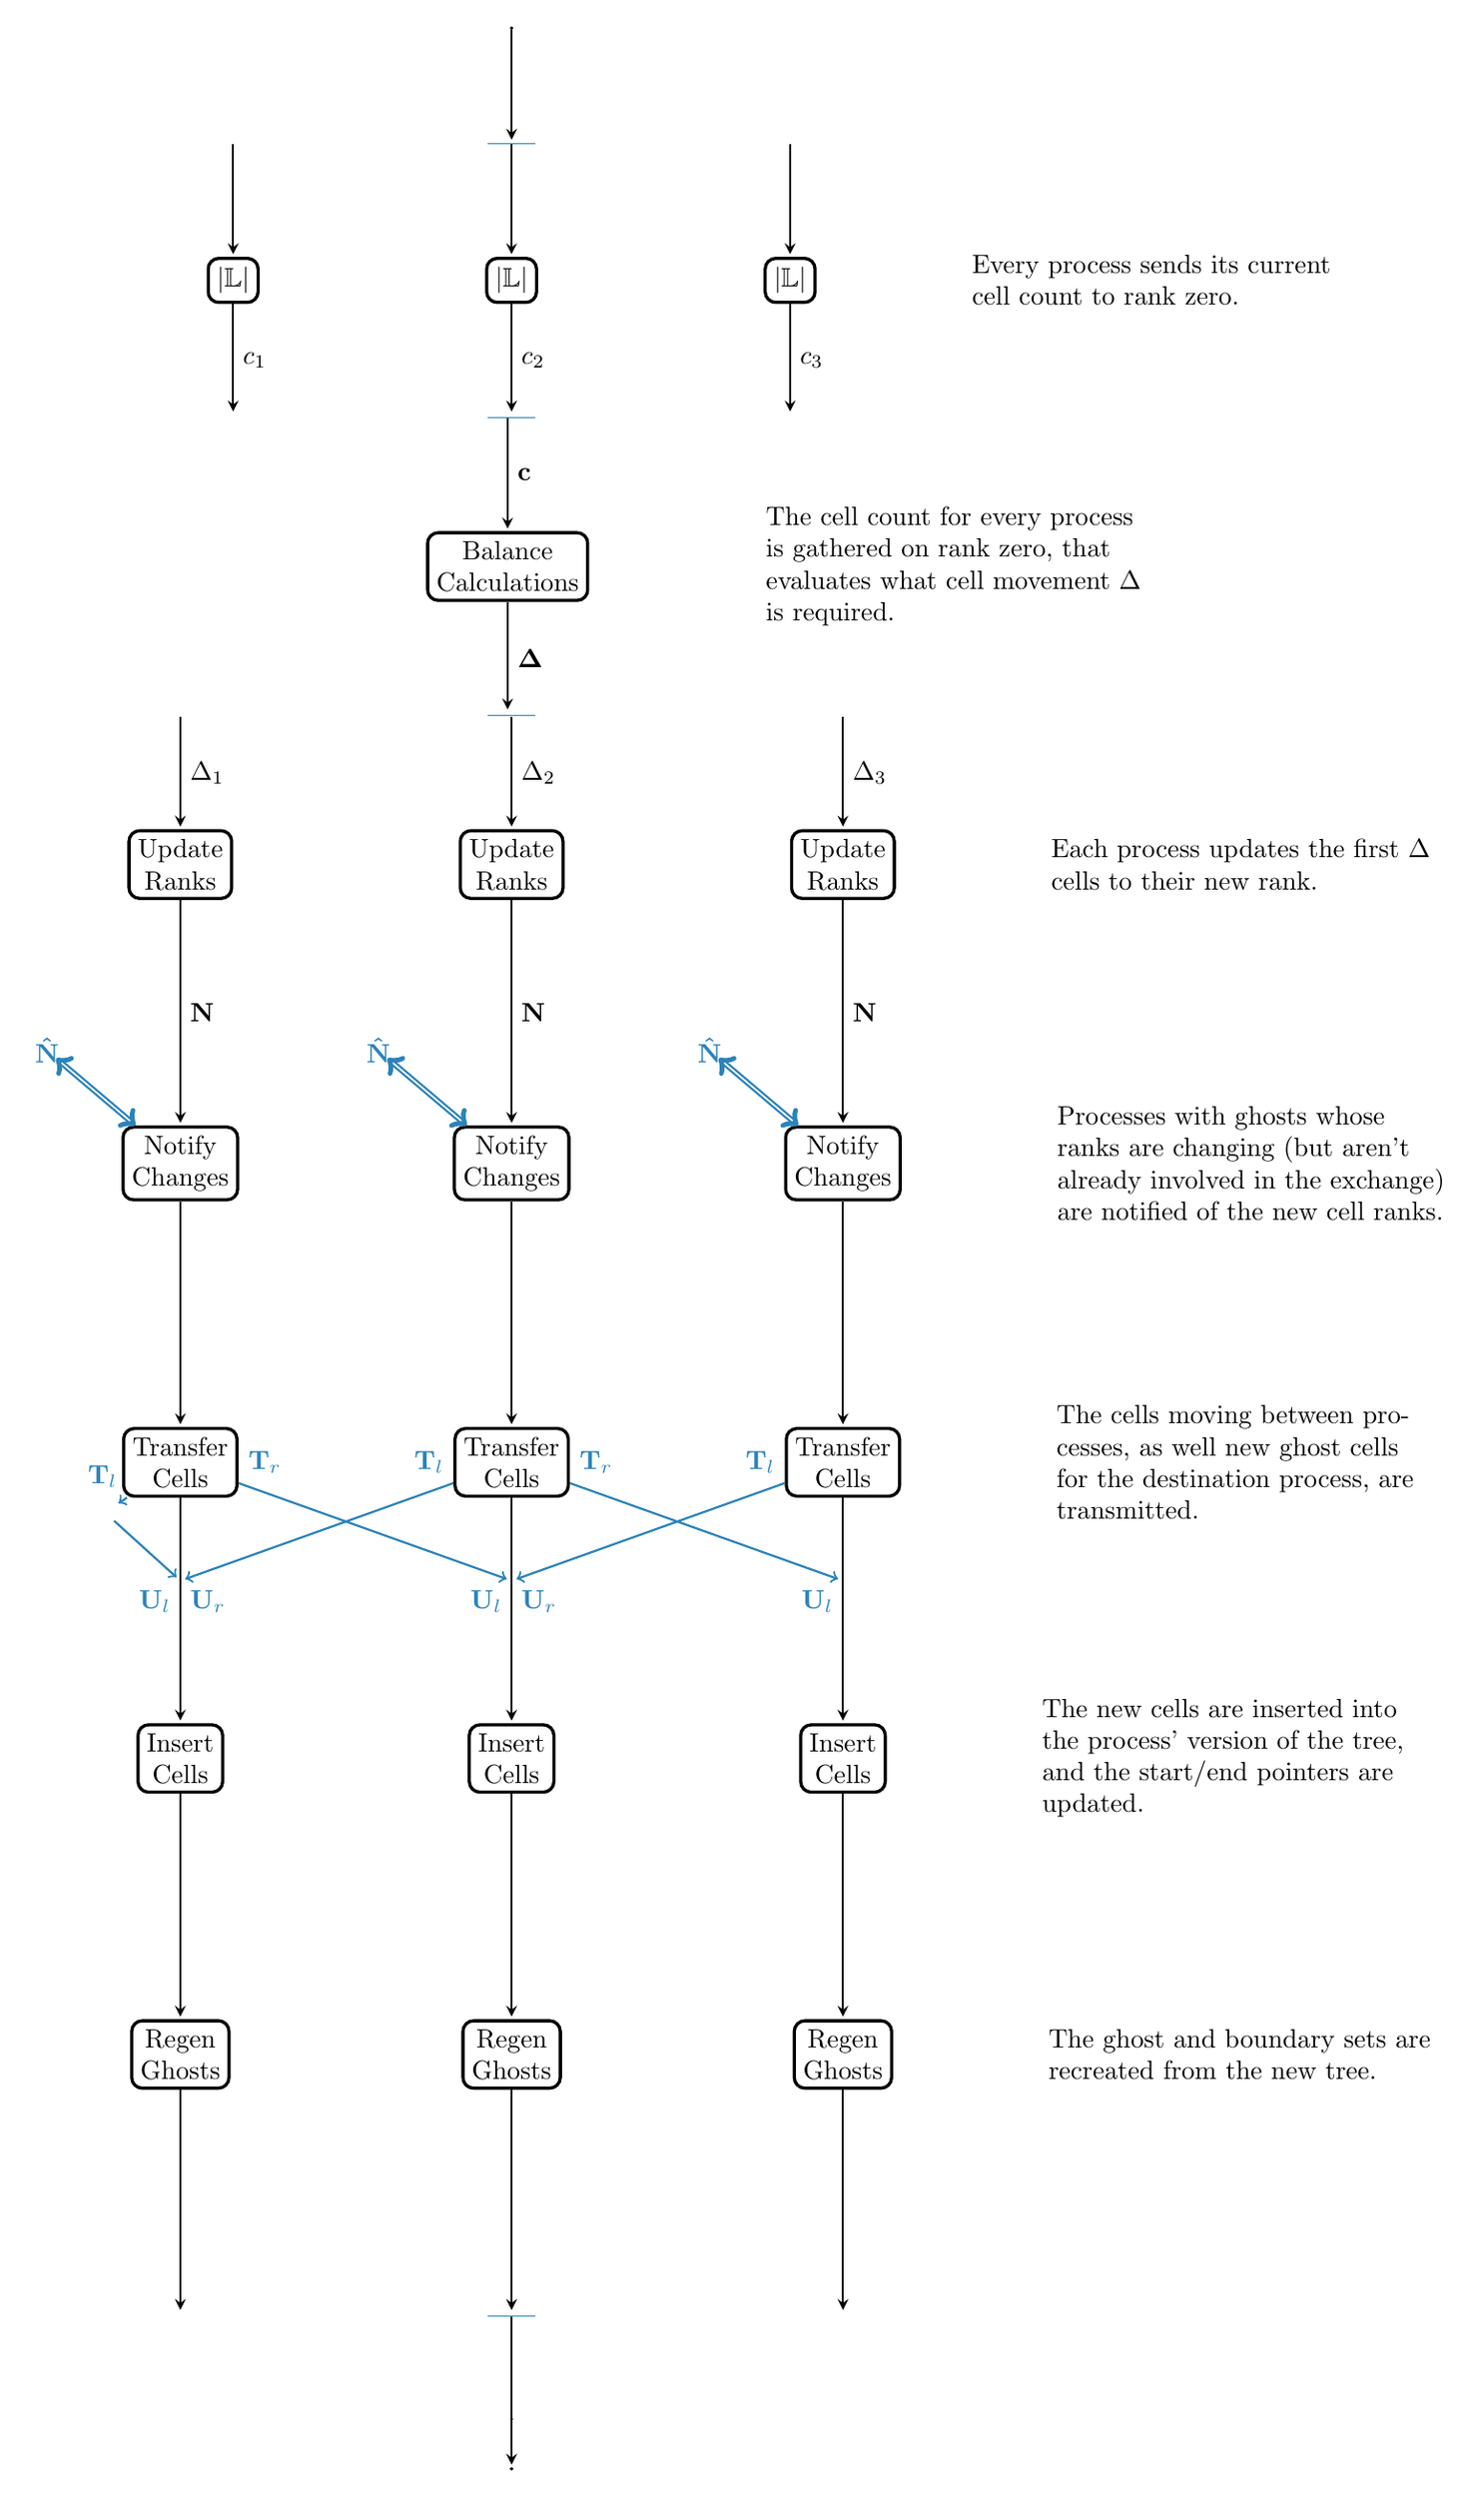
\begin{tikzpicture}[auto]
\pgftransformxscale{1.000000}
\pgftransformyscale{-1.000000}

\linespread{1}

\tikzset{
    adaction/.style={
        rectangle,
        rounded corners,
        draw=black,
        very thick,
        minimum width=4\du,minimum height=2\du,
        align=center
    },
    adedge/.style={->,
        >=stealth,
        shorten >=1pt,
        thick, 
        to path={(\tikztostart) -| (\tikztotarget)}
    },
    adforkedge/.style={->,
        >=stealth,
        shorten >=1pt,
        thick, 
        to path={
            (perpendicular cs: horizontal line through={(\tikztostart.south)},
                                     vertical line through={(\tikztotarget)}) 
            
            -- (\tikztotarget) \tikztonodes
        }
    },
    adjoinedge/.style={->,
        >=stealth,
        shorten >=2pt,
        thick, 
        to path={
            (\tikztostart)
            -- (perpendicular cs: horizontal line through={(\tikztotarget.north)},
                                 vertical line through={(\tikztostart)}) \tikztonodes
        }
    },
    adinit/.style={
        circle,
        draw,
        fill=black,
        inner sep=0,
        minimum size=0.8\du
    },
    adfinala/.style={
        circle,
        draw,
        inner sep=0,
        minimum size=0.8\du
    },
    adfinalb/.style={
        circle,
        draw,
        fill=black,
        inner sep=0,
        minimum size=0.6\du
    },
    adfork/.style={
        rectangle,
        fill=colorA,
        inner sep=0,
        minimum width=18\du,minimum height=0.25\du,
    },
    adcomms/.style={->,
        thick, colorA
    },
    adcommtarget/.style={
        draw=none,
        colorA
    }
}

\begin{scope}[
        node distance=2\du,
        every node/.style={}
]


\begin{scope}[
    node distance=1.5\du
]

\node[adinit] (init) {};
\node[adfork, below=of init] (f1) {};

\draw [adedge] (init) -- (f1);

\node[adaction, below=of f1] (r2-count) {$\abs{\mathbb{L}}$};
\node[adaction, left=3\du of r2-count] (r1-count) {$\abs{\mathbb{L}}$};
\node[adaction, right=3\du of r2-count] (r3-count) {$\abs{\mathbb{L}}$};

\end{scope}


\begin{scope}[
    node distance=1.5\du
]

\node[adfork, below=of r2-count] (f2) {};
\foreach \i in {1,2,3} {
    \draw [adforkedge] (f1) to (r\i-count);
    \draw [adjoinedge] (r\i-count) to node [anchor=west] {$c_\i$} (f2);
}

\node[adaction, below=of f2, xshift=-1.5\du] (balanceCalc) {Balance \\ Calculations};

\node[adfork, below=of balanceCalc, xshift=1.5\du] (f3) {};

\draw [adforkedge] (f2) to node [anchor=west] {$\vb{c}$} (balanceCalc);
\draw [adjoinedge] (balanceCalc) to node [anchor=west] {$\vb{\Delta}$} (f3);


\node[adaction, below=of f3] (r2-updateRanks) {Update \\ Ranks};
\node[adaction, left=3\du of r2-updateRanks] (r1-updateRanks) {Update \\ Ranks};
\node[adaction, right=3\du of r2-updateRanks] (r3-updateRanks) {Update \\ Ranks};

\end{scope}

\foreach \i in {1,2,3} {
    \draw [adforkedge] (f3) to node [anchor=west] {$\Delta_\i$} (r\i-updateRanks);

    \node[adaction, below=3\du of r\i-updateRanks] (r\i-notify) {Notify \\ Changes};
    \node[adaction, below=3\du of r\i-notify] (r\i-genSet) {Transfer \\ Cells};
    \node[adaction, below=3\du of r\i-genSet] (r\i-insert) {Insert \\ Cells};
    \node[adaction, below=3\du of r\i-insert] (r\i-ghosts) {Regen \\ Ghosts};

    \draw [adedge]
        (r\i-updateRanks.south) -- node [anchor=west] {$\vb{N}$} (r\i-notify.north);
    \draw [adedge]
        (r\i-notify.south) -- (r\i-genSet.north);
    \draw [adedge]
        (r\i-genSet.south) -- (r\i-insert.north);
    \draw [adedge]
        (r\i-insert.south) -- (r\i-ghosts.north);


    \node[adcommtarget, above left=1\du of r\i-notify] (r\i-n) {$\vb{\hat N}$};
    \draw[adcomms,double,<->,shorten >=-6pt] (r\i-notify) -- (r\i-n);

    \coordinate (r\i-mid) at ($(r\i-genSet)!0.4!(r\i-insert)$);
}


\node[adcommtarget, below left=0.1\du of r1-genSet, draw=none, xshift=-1\du] (r0-mid) {};

\draw[adcomms, shorten >=2pt] 
    (r1-genSet) -- (r0-mid)
    node [at start, above left] {$\vb{T}_l$};
\draw[adcomms, shorten >=2pt] 
    (r0-mid) -- (r1-mid)
    node [at end, below left] {$\vb{U}_l$};

% \node[adcommtarget, below right=0.1\du of r3-genSet, draw=none, xshift=1\du] (r4-mid) {};
% \draw[adcomms, shorten >=2pt] 
%     (r3-genSet) -- (r4-mid)
%     node [at start, above right] {$\vb{T}_r$};
% \draw[adcomms, shorten >=2pt] 
%     (r4-mid) -- (r3-mid)
%     node [at end, below right] {$\vb{U}_r$};


\draw[adcomms, shorten >=2pt] 
    (r1-genSet) -- (r2-mid)
    node [at start, above right] {$\vb{T}_r$}
    node [at end, below left] {$\vb{U}_l$};

\draw[adcomms, shorten >=2pt] 
    (r2-genSet) -- (r1-mid)
    node [at start, above left] {$\vb{T}_l$}
    node [at end, below right] {$\vb{U}_r$};

\draw[adcomms, shorten >=2pt] 
    (r2-genSet) -- (r3-mid)
    node [at start, above right] {$\vb{T}_r$}
    node [at end, below left] {$\vb{U}_l$};

\draw[adcomms, shorten >=2pt] 
    (r3-genSet) -- (r2-mid)
    node [at start, above left] {$\vb{T}_l$}
    node [at end, below right] {$\vb{U}_r$};
    

\node[adfork, below=3\du of r2-ghosts] (f4) {};

\foreach \i in {1,2,3} {
    \draw[adjoinedge] (r\i-ghosts) to (f4);
}

\node[adfinala, below=of f4] (finala) {};
\node[adfinalb, below=-0.7\du of finala] (finalb) {};

\draw [adedge] (f4) -- (finala);


\node[anchor=west, xshift=-1.6\du, right=of r3-count,text width=5.2cm] {
Every process sends its current cell count to rank zero.
};

\node[anchor=west, xshift=6.5\du, right=of balanceCalc,text width=5.2cm] {
The cell count for every process is gathered on rank zero, that evaluates what cell movement $\Delta$ is required.};

\node[anchor=west, xshift=-1.6\du, right=of r3-updateRanks,text width=5.2cm] {
Each process updates the first $\Delta$ cells to their new rank.};

\node[anchor=west, xshift=-1.6\du, right=of r3-notify,text width=5.2cm] {
Processes with ghosts whose ranks are changing (but aren't already involved in the exchange) are notified of the new cell ranks.
};

\node[anchor=west, xshift=-1.6\du, right=of r3-genSet,text width=5.2cm] {
The cells moving between processes, as well new ghost cells for the destination process, are transmitted.
};

\node[anchor=west, xshift=-1.6\du, right=of r3-insert,text width=5.2cm] {
The new cells are inserted into the process' version of the tree, and the start/end pointers are updated.
};

\node[anchor=west, xshift=-1.6\du, right=of r3-ghosts,text width=5.2cm] {
The ghost and boundary sets are recreated from the new tree.
};

\end{scope}

\end{tikzpicture}

\end{figure}


\subsubsection{Balance Calculation}
\label{sec:rebalancing-calc}

The cell counts $\vect{c}$ from each node are gathered on rank zero. Balancing is determined necessary based on a parameter $c_{crit}$ if $\norm{\vect{c}}>c_{crit}$. Algorithm \ref{alg:rebalance-calculatepassing} is then sufficient to determine the number of cells $\Delta$ each process passes left and right to balance every process to the average cell count $\bar c$. A negative value of $\Delta$ gives a cell count being received. 

The loop in Algorithm \ref{alg:rebalance-calculatepassing} can be reformulated as a proof by induction that the result is the minimum $\Delta$ satisfying the conditions imposed and $\abs{\mathbb{L}}_p=\bar c$ for all $p$.

\begin{algorithm}[H]
\caption{Rebalancing Calculations}
\label{alg:rebalance-calculatepassing}

\begin{algorithmic}
\Ensure For each process $p \in \mathbb{W}$ a pair of cell pass counts $\Delta_p = \{l,r\}$ where $l$ and $r$ are the number of cells to pass left and right respectively.
\Statex
% \Gather $\vect{c} \dla$ \Call{CellCount}{$p$}
\Gather $\vect{c} \dla \abs{\mathbb{L}}_p $
\ForEach {process $p \in \mathbb{W}$}
	\State $l_p \gets -r_{p-1}$
	\State $r_p \gets c_p - l_p - \bar{c}$
\EndFor
\end{algorithmic}
\end{algorithm}

Each process then receives from rank zero the two values in $\Delta_p$ which are enough to fully describe the following cell movements. 


\subsubsection{Update Cell Ranks}
\label{sec:rebalancing-updatecellranks}

Based on the movement amount $\Delta$ each process marks the cells to be moved with their new rank, storing the set of changes that would affect the ghost cells of other processes in order to notify them of the change in the next phase of rebalancing in Section \ref{sec:rebalancing-notifyrank}. The processes that need to be notified of changes is known by using the set of border cells $\mathbb{B}$. The process receiving the cells does not need to be notified of changes, as this data will be transmitted as part of the send sets in Section \ref{sec:rebalancing-gensendset}.

In the example case, the cells that are currently on rank 0 but will have their ranks updated to equal 1 are shown in red in Figure \ref{fig:rebalance-ranks}.

\begin{figure}[H]
	\caption{Example mesh, with 20 cells being marked to be moved from rank 0 to rank 1}
	\label{fig:rebalance-ranks}
	\input{method/gen/overlap.tex}
\end{figure}

\begin{algorithm}[H]
\caption{Updating Cell Ranks}
\label{alg:rebalance-updateranks}

\begin{algorithmic}
\Require Number of cells to pass left and right $\Delta = \{\Delta_l,\Delta_r\}$
\Ensure For each border $b$, a set $\vect{N}_b \in \{\lambda,r\}^n$ of pairs of cell identifiers $\lambda$ and new rank numbers $r$.
\Statex
\State $\vect{N} \gets \emptyset$
\ForEach {cell $\mathcal{C} \in \{\mathbb{L} : \text{in first }\Delta_l\} $}
	\Comment{For right, $\mathcal{C} \in \{\mathbb{L} : \text{in last }\Delta_r\} $}
	\State $\mathcal{C} \acc \textproc{rank} \gets p_{left}$
	\ForEach {process border $b \in \mathbb{W} \setminus \{p, p_{left}\}$}
		\If {$\mathcal{C} \in \mathbb{B}_b$}
			\State $\vect{N}_b \gets \{\mathcal{C} \acc \textproc{ident} , p_{left}\}$
		\EndIf
	\EndFor
\EndFor

\end{algorithmic}
\end{algorithm}

The routine in Algorithm \ref{alg:rebalance-updateranks} is repeated for the cells to move right, using the same sets $\vect{N}_b$.

In the example case, the only process not involved in the transfer already is the one at rank 2. The cells currently on rank 0, but being transferred to rank 1, that border it form the set $\vect{N}_2$ shown in Figure \ref{fig:rebalance-notify}.

\begin{figure}[H]
	\caption{The example mesh, with the ghost cells of rank 2 whose rank will change following the rebalancing highlighted}
	\label{fig:rebalance-notify}
	\input{method/gen/ghostnotify.tex}
\end{figure}


\subsubsection{Notifying Rank Changes}
\label{sec:rebalancing-notifyrank}

The rank change lists stored in the previous section are now sent. Each process then receives all the changes relevant to its ghosts according to Algorithm \ref{alg:rebalance-notifyranks}. 

This rank change stage needs to occur before the cells are moved to the new process, as the receiving process is not guaranteed to have the relevant border data required. 

\begin{algorithm}[H]
\caption{Notifying Cell Rank Changes}
\label{alg:rebalance-notifyranks}

\begin{algorithmic}
\Require For each border $b$, a set $\vect{N}_b \in \{\lambda,\rho\}^n$ of pairs of cell identifiers $\lambda$ and new rank numbers $\rho$.
\Statex
\ForEach {process border $b \in \mathbb{W} \setminus p$}
	\Send $N_b \dra p_b$
\EndFor
\Statex
\ForEach {process border $b \in \mathbb{W} \setminus p$}
	\Recv $\hat N_b \dla p_b$
	\ForAll {$\{\lambda,\rho\} \in \hat N_b$}
		\State $\mathcal{C}\gets\textproc{Find}(\lambda)$
		\State $\mathcal{C}\acc\textproc{rank} \gets \rho$
	\EndFor
\EndFor
\end{algorithmic}
\end{algorithm}


\subsubsection{Generate Send Sets}
\label{sec:rebalancing-gensendset}

After notifying the foreign processes of rank changes, each process then generates the set of cell required to be sent. In addition to the cells being moved, cells in their poisson neighbourhoods not on the rank of the receiving process must also be included in the sets as seen in Figure \ref{fig:rebalance-transfer}.

\begin{figure}[H]
	\caption{The example mesh, with the cells of $T_r$ highlighted}
	\label{fig:rebalance-transfer}
	\input{method/gen/Tr.tex}
\end{figure}

\begin{algorithm}[H]
\caption{Generate Send Sets}
\label{alg:rebalance-gensendsets}

\begin{algorithmic}
\Require Number of cells to pass left $\Delta_l$
\Ensure A set of packed cells $\vect{T}_l \in \{\lambda, \rho, \phi\}^n$ containing the cell's identifiers $\lambda$, rank $\rho$ and data $\phi$.
\Statex
\State $\vect{T}_l \gets \emptyset$
\ForEach {cell $\mathcal{C} \in \{\mathbb{L} : \text{in first }\Delta_l\} $}
	\Comment{If sending right, $\mathcal{C} \in \{\mathbb{L} : \text{in last }\Delta_r\} $}
	\State $T_l \gets \{\mathcal{C}\acc\textproc{ident}, \mathcal{C}\acc\textproc{rank}, \mathcal{C}\acc\textproc{data}\}$

	\ForEach {cell $\mathcal{P} \in \mathcal{C}\acc\vect{\mathcal{P}}$}
		\Comment{$\mathcal{C}\acc\vect{\mathcal{P}}$ is the poisson neighbours of $\mathcal{C}$}
		\If {$\mathcal{P}\acc\textproc{rank} \neq p_{left}$}
			\State $T_l \gets \{\mathcal{P}\acc\textproc{ident}, \mathcal{P}\acc\textproc{rank}, \mathcal{P}\acc\textproc{data}\}$
		\EndIf
	\EndFor
\EndFor
\end{algorithmic}
\end{algorithm}

The two sets $T_l$ and $T_r$ are then transmitted left and right respectively, and the corresponding sets from the foreign processes $U_l$ and $U_r$ are received. 

\begin{algorithm}[H]
\caption{Send Sets}
\label{alg:rebalance-sendsets}

\begin{algorithmic}
\Require A set of packed cells $\vect{T}_l \in \{\lambda, \rho, \phi\}^n$ containing the cell's identifiers $\lambda$, rank $\rho$ and data $\phi$.
\Statex
\Send $\vect{T}_l \dra p_{left} \qquad\ \,;\qquad \algorithmicsend\ \vect{T}_r \dra p_{right}$
\Recv $\vect{U}_r \dla p_{right} \qquad;\qquad \algorithmicrecv\ \vect{U}_l \dla p_{left}$
\end{algorithmic}
\end{algorithm}

The combined set $\vect{U}=\vect{U}_l\cup\vect{U}_r$ now contains all the additional information required by the process that wasn't available prior.  

\subsubsection{Insert Cell Set}
\label{sec:rebalancing-insertcells}

Each process then inserts the received cells in $\vect{U}$ and calculates the poisson neighbourhood. All the new cells must be inserted before calculating poisson neighbourhoods, as the correct neighbourhood may include new cells that wouldn't exist prior.

\begin{algorithm}[H]
\caption{Insert Received Cells}
\label{alg:rebalance-insertset}

\begin{algorithmic}
\Require A set of received packed cells from the right $\vect{U} \in \{\lambda, \rho, d\}^n$ containing the cell's identifiers $\lambda$, rank $\rho$ and data $\phi$.
\Statex
\State $\vect{\Gamma} \gets \emptyset$ \Comment{Cache the cells corresponding to $\vect{U}$}
\ForEach {packed cell $\{\lambda, \rho, \phi\} \in \vect{U}$}
	\State $\mathcal{C} \gets \Call{Insert}{\lambda}$
	\State $\mathcal{C}\acc\textproc{rank} \gets \rho \qquad;\qquad \mathcal{C}\acc\textproc{data} \gets \phi$
	\State $\vect{\Gamma} \gets \mathcal{C}$
\EndFor
\Statex
\ForEach {cell $\mathcal{C} \in \vect{\Gamma}$}
	\State $\mathcal{C}\acc\{\vect{\mathcal{P}}, \vect{b}, \alpha \} \gets \textproc{CalcPoisCoefs}(\mathcal{C})$
\EndFor
\end{algorithmic}
\end{algorithm}


\subsubsection{Regenerate Ghosts}
\label{sec:rebalancing-regenghosts}

The subset of the tree in each process now shows the completed transfer as in Figure \ref{fig:rebalance-final} for the example case. The ghost and border sets are now outdated however, so must be amended.

\begin{figure}[H]
	\caption{The rebalanced example mesh}
	\label{fig:rebalance-final}
	\input{method/gen/result.tex}
\end{figure}


Although enough information exists to work out the changes required to be made to the border and ghost sets, it is much simpler in practice to reconstruct them completely. Since rebalancing is performed irregularly, the performance cost is negligible. 

The method for reconstruction is equivalent to Algorithm \ref{alg:distrib-ghosts}, but since all cells in $\mathbb{L}$ have rank $p$ the result is the ghost set for the current context. Border cells are regenerated exactly as in Algorithm \ref{alg:borders-gen}.


% \section{Results}

% \subsection{Boundary size for Hilbert Curve}
% \label{sec:boundarysize}

% It is possible to test the size of the boundary for different practical scenarios when using The Hilbert Curve to distribute. This is done for a complex and finely detailed geometry (the Mandelbrot example) as well as a more simple geometry with smooth edges. 

% Boundary sizes need min/max/mean relative to cell count for many configurations.

% Comparison points of other space filling curves.

% Description of optimal method.

% \subsection{Performance against Thread Count}

% \subsection{Cluster Operation Above Single Node Memory Limit}

% \section{Conclusion}

% \printbibliography

\end{document}
